%! Author = Philipp Emmenegger
%! Date = 29/06/2021

\section{Reverse Engineering}
Software Reverse Engineering helps:
\begin{itemize}
    \item understand malware
    \item understand legacy code
    \item remove usage restriction from software
    \item fond and exploit flaws 
    \item cheat at games
\end{itemize}

\subsection{Compiling}
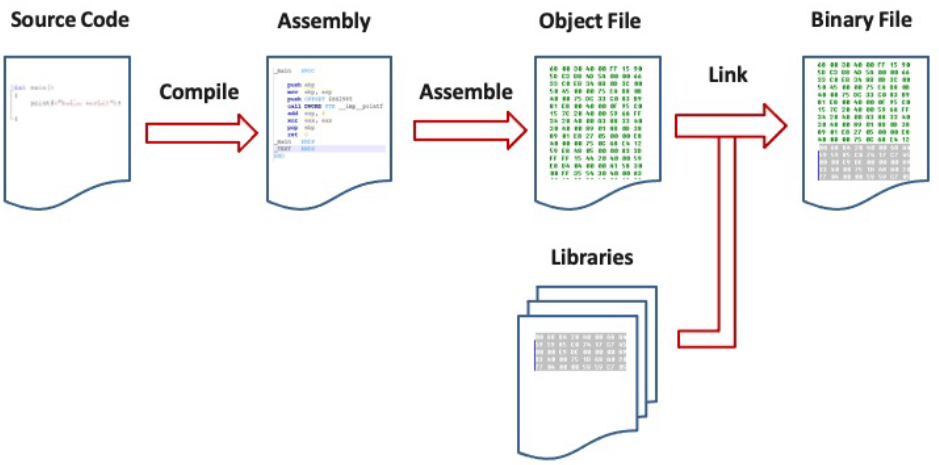
\includegraphics[width=\linewidth]{../img/compiling.png}

\subsection{Loading}
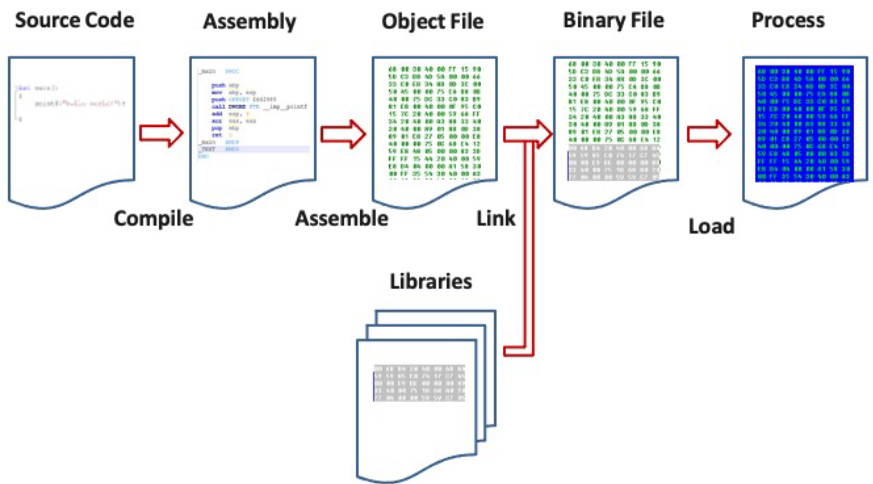
\includegraphics[width=\linewidth]{../img/loading.png}

\subsection{Running}
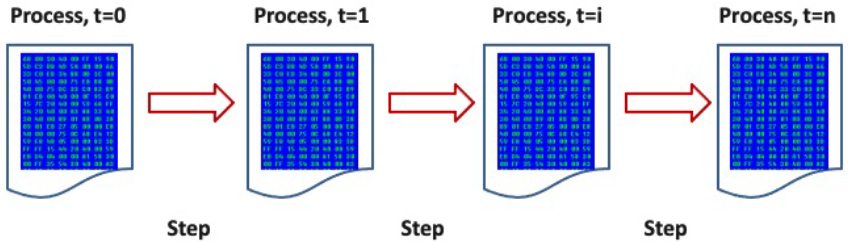
\includegraphics[width=\linewidth]{../img/running.png}

\subsection{Reverse Engineering Domain}
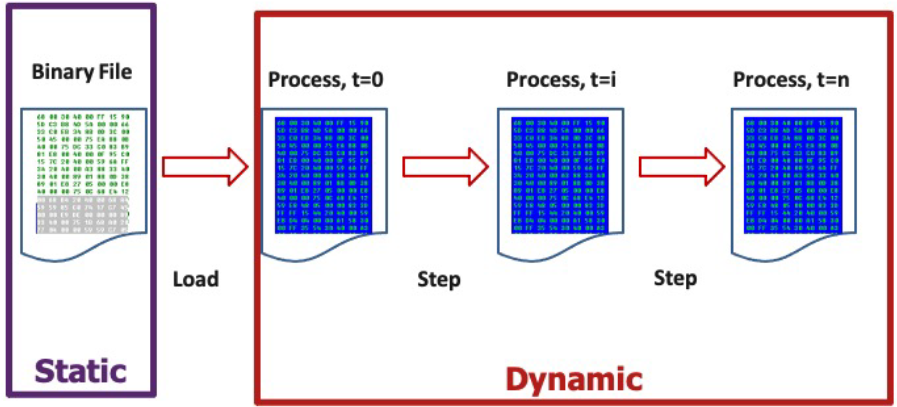
\includegraphics[width=\linewidth]{../img/reverse_engineering_domain.png}

\subsection{Tools}
\textbf{Disassembler}
\begin{itemize}
    \item Converts exe to assembly (as best as it can)
    \item Cannot always disassemble 100\% correctly
    \item Not possible to reassemble into working exe
    \item Gives static results
    \item Good overview of program logic
    \item Difficult to jump to specific place in the code
\end{itemize}
\textbf{Debugger}
\begin{itemize}
    \item Step thru code to understand it
    \item Labor intensive
    \item Can set break points
    \item Can treat complex code as black box
\end{itemize}
\textbf{Hex editor}
\begin{itemize}
    \item Patch (modify) exe file
\end{itemize}
\textbf{Process Monitor, VMware, ...}

\subsection{Mitigations against Reverse Engineering}
\begin{itemize}
    \item Impossible to prevent
    \item Possible to make it more difficult
    \begin{enumerate}
        \item Anti-disassembly: confuse static view of code
        \item Anti-debugging: confuse dynamic view of code
        \item Tamper resistance: code checks itself to detect tampering
        \item Code obfuscation: make code more difficult to understand
    \end{enumerate}
\end{itemize}

\columnbreak
\subsubsection{Anti Dissasembly}
\begin{itemize}
    \item Encrypted or packed object code
    \item False disassembly
    \item Self-modifying code
    \item Encryption prevents disassembly
\end{itemize}

\subsubsection{Anti Debugging}
\begin{itemize}
    \item \textit{IsDebuggerPresent()}
    \item Monitor for debug registers / breakpoints
    \item Debuggers do not handle threads well
\end{itemize}
\textbf{Example:}
\begin{itemize}
    \item Programs gets \textit{inst 1} and pre fetches following
    \item Debugger does not pre-fetch
    \item Overwrite later instruction after pre fetching
    \item Program without debugger will be okay
    \item Only works if segment of code is executed once
\end{itemize}

\subsubsection{Tamper Resistance}
\begin{itemize}
    \item Make patching more difficult
    \item Code can hash parts of itself, hash checks later
    \item This approach is called \textit{guards}
\end{itemize}

\subsubsection{Code Obfuscation}
\begin{itemize}
    \item Make code hard to understand
    \item Opposite of good software engineering
    \item spaghetti code
\end{itemize}
\begin{lstlisting}
int x,y;
if((x-y)*(x-y) > (x*x-2*x*y+y+y)) { } // always true
\end{lstlisting}
\textbf{Code Bloating:}
\begin{enumerate}
    \item Insert dead code
    \item Adding zero effect operations
    \item Transform the data (ASCII Chars instead of numbers)
\end{enumerate}